\section[Potentials]{Exactly Solvable Potentials}

\subsection[Infinite Well]{The Infinite Square Well}

\begin{frame}{The Infinite Square Well}
	Here the potential is of the form
	\[
		V(x) = \begin{cases}
			0      & 0 \leq x \leq a  \\
			\infty & \text{otherwise}
		\end{cases}
	\]
	And as a consequence the Schrödinger equation looks like
	\begin{align*}
		-\frac{\hbar^2}{2m} \dv[2]{\psi}{x} = E \psi &  & \dv[2]{\psi}{x} = -\frac{2mE}{\hbar^2 } \psi    \\
		\dv[2]{\psi}{x} -k^2 \psi                    &  & \text{where } k \equiv \frac{\sqrt{2mE}}{\hbar}
	\end{align*}
	Because $E$ must be at least greater than the smallest $V(x)$, $E\ge 0$ and the solution is of the form
	$$ \psi(x) = A \sin kx + B \cos kx$$

	Now we apply boundary conditions  like $\psi(0) = \psi(a) = 0$ and $\psi(x)$ is continuous. We find that $B = 0$ and
	$$ \boxed{k = k_n = \frac{n \pi}{a} \to E_n = \frac{\hbar^2 k_n^2}{2m} = \frac{\hbar^2 n^2 \pi^2}{2ma^2}} $$

\end{frame}

\begin{frame}
	Now we must find $A$ via the normalization condition.
	$$ \int_0^a |A|^2 \sin[2](kx) \dd{x} = |A|^2 \frac a2 = 1 \qq{so} |A|^2 = \frac 2a$$ We pick the positive real value of $A$ and have that
	$$ \psi_n(x) = \sqrt{\frac{2}{a}} \sin(\frac{n \pi}{a}x)$$
	The lowest energy state is $\psi_1$, called the ground state. The next is $\psi_2$ and so on. Each has energy that is $E_n \propto n^2$ and as a collection, the functions $\psi_n(x)$ have the following properties.

\end{frame}

\begin{frame}{Some notes on $\psi_n(x)$}
	\begin{enumerate}
		\item They are alternately even and odd, with respect to the center of the well: $\psi_1$ is even, $\psi_2$  is odd, $\psi_3$ is even,and so on. True when $V(x)$ is a symmetric function.
		\item As you go up in energy, each state has more nodes according to the figure below(edges don't count). This is universal.
		\item They are mutually orthogonal i.e. $\displaystyle \int \psi_m(x)^* \psi_n(x) \dd x = 0, (m \neq n)$. And in general $$\int \psi_m(x)^* \psi_n(x) \dd{x} = \delta_{mn}$$
	\end{enumerate}

	\begin{figure}
		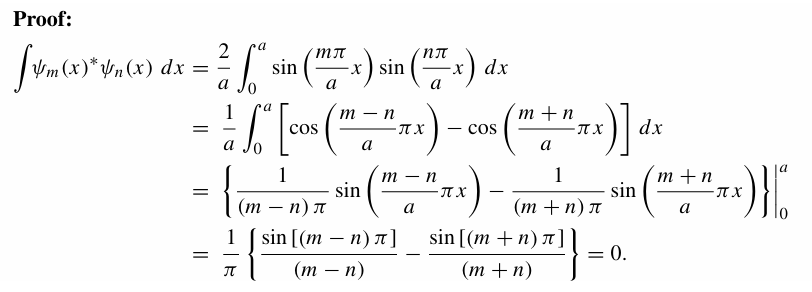
\includegraphics[width = .9\linewidth,trim=0cm 0 0 4mm]{QM_proof1.png}
	\end{figure}

\end{frame}

\begin{frame}{More notes}
	\begin{enumerate}
		\setcounter{enumi}{3}
		\item They are \textbf{complete} i.e. any function can be expressed in terms of linear combinations of $\psi_n(x)$. (This is practically always true but not in general...) $$ f(x) = \sum_{n=1}^{\infty} c_n \psi_n(x)	= \sqrt{\frac 2a } \sum_{n=1}^{\infty} c_n \sin(\frac{n\pi}{a} x)$$ (sometimes called the Dirichlet Theorem). Using Fourier's trick we can get the coefficient $c_n$ to be  $$ c_n = \int \psi_n(x)^* f(x) \dd{x} $$
	\end{enumerate}
\end{frame}

\begin{frame}{Back to the square well}
	The stationary states for the square well are
	\[
		\Psi_n(x,t) = \sqrt{\frac 2a} \sin(\frac{n\pi}{a}x) \exp(-i \frac{n^2\pi^2 \hbar^2}{2ma^2}t)
	\]
	(remember the time factor from eq. \ref{eq:GeneralSol}) and therefore the general solution for the infinite square well is
	\begin{equation}
		\label{eq:sol_sqwell}
		\Psi(x,t) = \sum_{n=1}^{\infty}c_n \sqrt{\frac 2a} \sin(\frac{n\pi}{a}x)e^{-i (n^2\pi^2 \hbar^2/2ma^2)t}
	\end{equation}
	With the $c_n$ to be
	\begin{equation}
		c_n = \sqrt{\frac 2a} \int_{0}^{a} \sin(\frac{n\pi}{a}x) \Psi(x,0) \dd{x}
	\end{equation}

\end{frame}

\subsection{Harmonic Oscillator}
\begin{frame}{The Harmonic Oscillator}
	The potential has the form $$ V(x) = \frac 12 kx^2 = \frac 12 m\omega^2 x^2$$ giving us the following TISE
	$$-\frac{\hbar^2}{2m} \dv[2]{\psi}{x} + \frac 12 m\omega^2x^2 \psi = E \psi$$
	This can be solved in 2 ways : Algebraic (using ladder operators) and Analytic  (power series solution).
	First the Algebraic method
\end{frame}
\begin{frame}{Algebraic method (Ladder operators)}
	We rewrite the TISE in the following form
	\[
		\frac{1}{2m} \qty[\hat{p}^2 + (m\omega x)^2]\psi =E\psi
	\]
	and invoke the ladder operators (I write it here in two equivalent forms Griffiths' and Sakurai's)

	\textbf{Note} $a_+ = a^\dag$ so $a_- = a$ in Sakurai's notation


	\begin{align*}
		\hat{a}_{\pm} = \frac{1}{\sqrt{2\hbar m \omega }} (m\omega x \; \mp i \hat p) &  & \hat{a}_{\pm} = \sqrt{\frac{m\omega}{2\hbar}} \qty(x \mp \frac{i p }{m\omega})
	\end{align*}

\end{frame}
